\documentclass[cn,10pt,math=newtx,citestyle=gb7714-2015,bibstyle=gb7714-2015]{elegantbook}
\lstset{language=bash} 

\setcounter{tocdepth}{0}
\title{Foreign Language Text Reader(FLTR)}
\subtitle{一个方便的语言学习的应用程序}

%\author{Ethan Deng \& Liam Huang}
%\institute{Elegant\LaTeX{} Program}
\date{\today{}}
\version{1.4.0 (2021-06-14)}
\bioinfo{译者}{\href{https://github.com/wuyudi/}{AsukaMinato}}

\extrainfo{Copyright \copyright  2012-2021 FLTR Developers et al.}

%\logo{logo-blue.png}
\cover{image/images-000_1.png}

% 本文档命令
\usepackage{array}
\usepackage[tikz]{bclogo}
\newcommand{\ccr}[1]{\makecell{{\color{#1}\rule{1cm}{1cm}}}}
\newcommand{\goldendict}{\href{http://goldendict.org/}{GoldenDict}}
\newcommand{\translateshell}{\href{https://github.com/soimort/translate-shell}{translate-shell}}
\usepackage{tabularx}
\definecolor{customcolor}{RGB}{32,178,170}
\colorlet{coverlinecolor}{customcolor}

\begin{document}

\maketitle
\frontmatter

\tableofcontents

\mainmatter
\setlength{\parskip}{2em}

\chapter*{译者言}

\href{https://www.zhihu.com/people/L.M.Sherlock}{叶哥}介绍了 \href{http://www.lingq.com/}{LingQ},然后我在 \url{https://alternativeto.net/} 找到了替代品  \href{http://lwt.sourceforge.net/}{Learning With Texts(LWT)}, 但是配置很麻烦,用了一阵子弃用。最后找到了 \href{https://sourceforge.net/projects/foreign-language-text-reader/}{FLTR}, 经过配置很好用。顺便汉化了手册。模板为 \href{https://github.com/ElegantLaTeX/ElegantBook}{ElegantBook} 。书中图片为用 \href{https://man.archlinux.org/man/pdfimages.1.en}{pdfimages} 从原手册提取的,封面图用 \href{https://www.gimp.org/}{GIMP} 修改了。使用 \href{https://www.deepl.com/translator/files}{DeepL} 初翻,人工校对。写作平台 \href{https://www.overleaf.com/}{Overleaf}, XeLaTeX, texlive 2021, 许可证遵循 FLTR 的许可证。

\chapter{摘要和介绍}

FLTR(= Foreign Language Text Reader)帮助你以轻松愉快的方式实现泛读与精读,作为你的外语学习的一部分。


在阅读时,你可以通过网络浏览器或本地安装的词典应用程序在词典中查找未知的单词,并保存词汇(单词和词组)的翻译、罗马化(如拼音、平假名等,可选)和例句(可选)。每个术语都有一个学习状态(1/"未知"到5/"已知",加上 "忽略 "和 "熟知 "的状态),并有相关的颜色。

保存的单词将自动显示其所有数据和状态,并在同一语言的所有文本中出现。它们可以通过导出功能轻松地导入到闪卡软件中,如\href{http://ankisrs.net/}{Anki}或\href{http://www.mnemosyne-proj.org/}{Mnemosyne}。


FLTR在许多方面与公共领域的软件 \href{http://lwt.sourceforge.net/}{"Learning With Texts"(LWT)}相似。但FLTR更容易安装和运行--不需要个人网络服务器,也不需要数据库。\href{http://www.lingq.com/}{"LingQ.com "}提供的网络服务有一个巨大的文本库、辅导服务和一个论坛,也与FLTR相当相似,但由于是网络服务,速度要慢得多。你必须在线才能使用LingQ,而且它需要付费(每月10美元)。更重要的是,你完全依赖于LingQ服务的可用性,而且你并不拥有你的词汇数据。如果你停止付费,你几乎会失去一切。
另请参见"\nameref{比较类似软件(FLTR, LWT, LingQ)}"

FLTR是用Java 1.8编程的,也被称为Java 8。要运行FLTR,你需要一个已安装的Java Runtime Engine(JRE),从\href{http://java.com}。该程序可在MacOS、Windows和Unix/Linux上运行。使用FLTR时不需要在线,但是如果你使用在线词 典,你必须在线。


FLTR以UTF-8文本或以TAB分隔的CSV文件读取和写入其数据(定义语言、文本、单词、导出、常规设置),这使得使用简单的程序如文本编辑器或电子表格程序来添加、更改或提取数据变得很容易。
\chapter{本软件的动机}
摘自\href{http://en.wikipedia.org/wiki/Extensive_reading}{维基百科 "广泛阅读"}一文。
\begin{quotation}

广泛阅读(或自由自愿阅读)是通过大量的阅读来帮助语言学习,包括外语学习。学习者在具体的 语境中查看和复习未知的单词,可以让学习者推断,从而学习这些单词的含义 。 ...广泛的阅读与精读形成鲜明对比的是,精读是指缓慢、仔细地阅读少量难懂的文章-是指 "专注于语言,而不是文本 "的时候。广泛阅读和精 读是语言学习和教学的两种方法,可以同 时使用;但精读是更常见的方法,而且往往是唯一使用的方法。
\end{quotation}
\href{https://zh.wikipedia.org/zh-hans/史蒂芬·克拉申}{斯蒂芬-克拉申}已经发表了350多篇论文和书籍,对第二语言习得、双语教育和阅读领域做出了贡献。


他提倡在第二语言学习过程中使用 "自由自愿阅读",他说这是 "我们在 语言教育中最有力的工具,无论是第一语言还是第二语言"。


观看\href{http://www.youtube.com/watch?v=NiTsduRreug}{这段视频}。


\href{https://blog.thelinguist.com/}{史蒂夫-考夫曼}创造了1400多个关于阅读(和听)在语言学习中的重要性的视频。

在YouTube上观看\href{https://www.youtube.com/user/lingosteve/videos?sort=p&flow=grid&view=0}{他的视频。}
\chapter{屏幕截图}

请注意,有些截图是用旧版本的软件制作的,没有更新。


主窗口(Windows 10,系统外观和感觉,130 \%)。

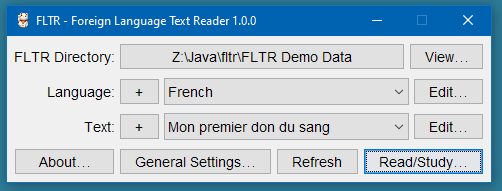
\includegraphics[scale=0.8]{image/images-006.png}

主窗口 (Linux Mint, 系统外观和感觉, 120 \%)

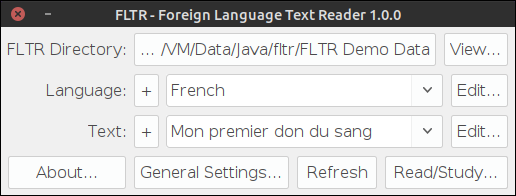
\includegraphics[scale=0.8]{image/images-007.png}


主窗口 (Linux, Nimbus Look \& Feel, 100 \%)

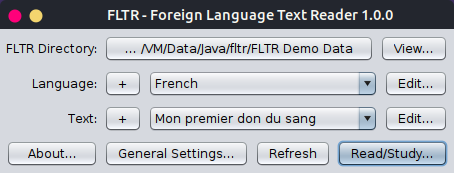
\includegraphics[scale=0.8]{image/images-009.png}


目录和文件结构

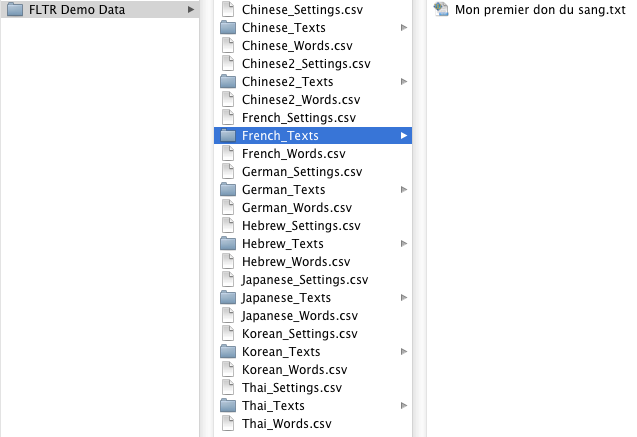
\includegraphics[scale=0.5]{image/images-011.png}

文本和词汇 Windows (Windows 10, 系统外观, 130 \%)

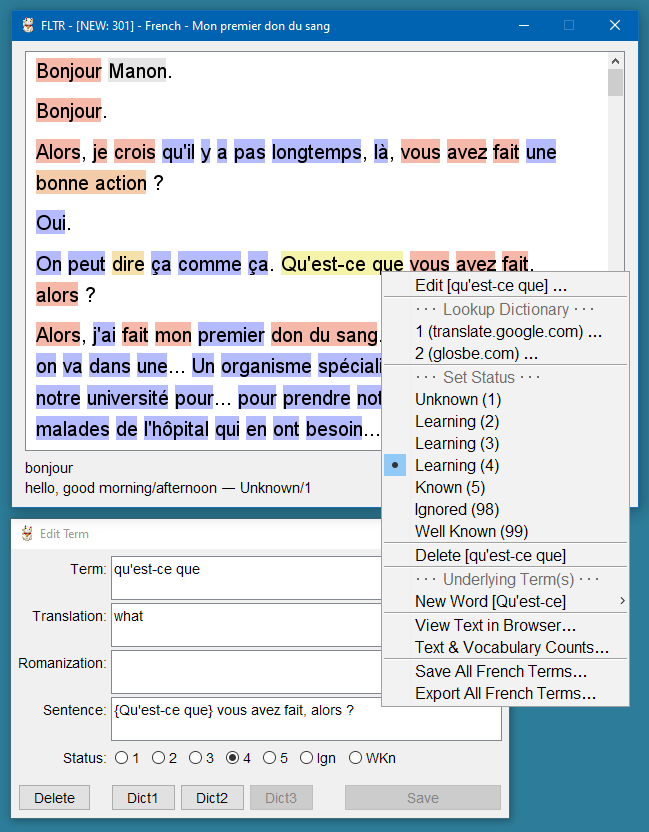
\includegraphics[scale=0.5]{image/images-012.png}


文本和词汇 Windows (Linux Mint, 系统外观, 100 \%)

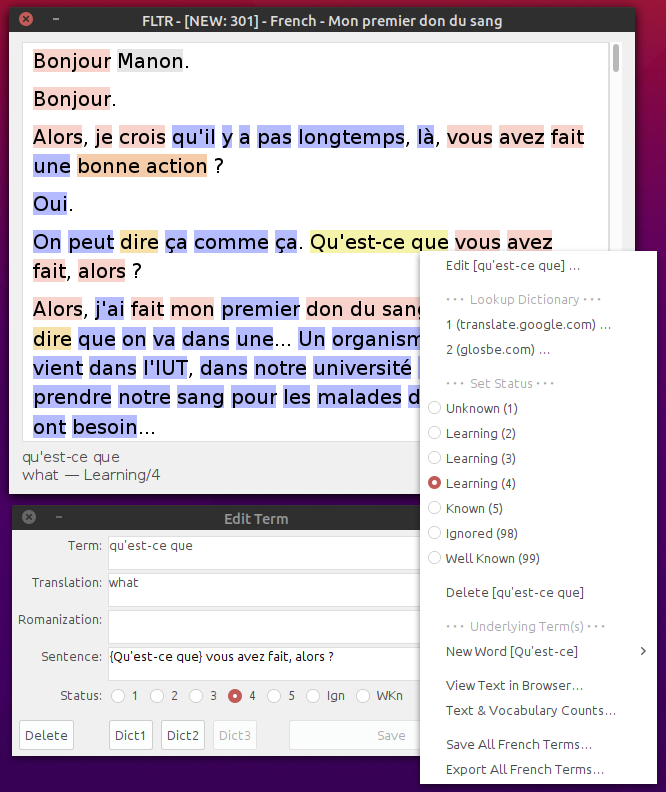
\includegraphics[scale=0.5]{image/images-013.png}

文本和词汇 Windows (Linux, Nimbus Look \& Feel, 100 \%)

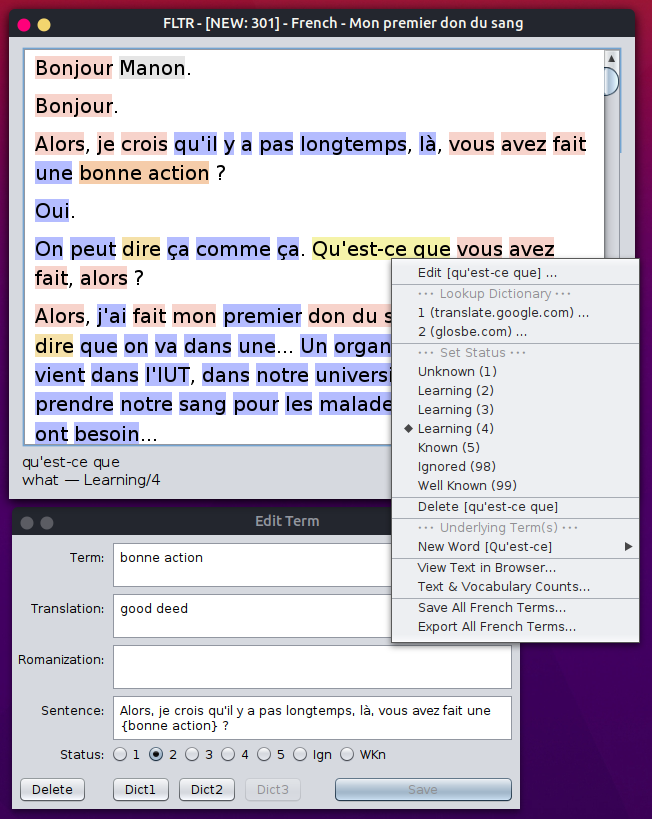
\includegraphics[scale=0.5]{image/images-014.png}



\chapter{ 概述}
\begin{itemize}
\item 第一件事:"\nameref{下载和安装}"。
\item 现在你必须进行 "\nameref{FLTR初始配置}"。
\item 语言设置将被保存在"XXX\_Settings.csv"(其中XXX是一种语言的名称)。这些设置必须为异国语言进行调整/改变,以便指定字典URL或程序调用、字体名称、字体大小等。见。"\nameref{FLTR语言设置} "和 "\nameref{与字典查询软件整合}"。
\item 一般的FLTR设置,如窗口大小等,被保存在用户的主目录下一个名为".prefs "的文件中。见。"\nameref{常规设置}"。
\item 现在,有趣的事情开始了。"\nameref{阅读文本,创造和编辑词语或表达方式}"。
\item 词汇将被保存在 "XXX\_Words.csv "中。可选的词汇导出将被保存在"XXX\_Export.txt "中。详情见。"\nameref{词汇文件}"。
\item 你可以用你保存的词汇进行工作。只要在文本组合框中选择<词汇>,然后对词汇进行过滤、排序和限制,并决定是以文本形式复习,还是在浏览器中复习,或者导出数据。见。"\nameref{复习和编辑词汇}。
\item 没有回答所有问题?请阅读 "\nameref{常见问题解答(FAQ)}"。
\item 最后。"\nameref{比较类似软件(FLTR, LWT, LingQ)}"和 "\nameref{版本历史}"。

\end{itemize}

\chapter{下载和安装}\label{下载和安装}

\section*{步骤1:}
检查你是否已经安装了Java。
\begin{itemize}
    \item 在命令或终端窗口中输入 \lstinline{java -version},可以看到已安装的Java版本号,如果没有安装Java,则会出现错误信息。
    \item  FLTR需要Java 1.8版本(又称Java 8)或更高版本。
\end{itemize}

\section*{步骤2:}
如果你的电脑上没有Java,请下载并安装Java。
\begin{itemize}
    \item 转到 \url{http://www.java.com/en/download/manual.jsp}
    \item 下载适合你的操作系统的版本。
    \item 安装它。
    \item 重复第1步,检查Java是否正确安装。
    \item 建议安装最新的可用版本。
\end{itemize}

\section*{步骤3:}
 下载并安装FLTR。
\begin{itemize}
    \item   转到 \url{https://sourceforge.net/projects/foreign-language-text-reader/files/} 
    \item 下载最新的压缩文件。
    \item 将其解压在你选择的目录中。
\end{itemize}

\section*{步骤4:}
启动FLTR。
\begin{itemize}

\item 双击
 \begin{itemize}\item FLTR.exe(仅适用于Windows)或FLTR.jar(适用于所有操作系统)。
 \end{itemize}

    \item 重要的是。在Linux、UNIX、macOS等系统中,FLTR.jar必须被设置为"可执行",以便由Java Runtime系统运行。( 只需在终端运行\lstinline{chmod a+x FLTR.jar}即可。)
    \item 你也可以通过命令行启动FLTR: \lstinline{java -jar FLTR.jar}
       
\end{itemize} 

阅读更多关于开始使用和配置FLTR的信息:"\nameref{FLTR初始配置}"


\chapter{FLTR初始配置}
\label{FLTR初始配置}
创建一个FLTR数据目录。

通过双击FLTR.exe或FLTR.jar启动FLTR。

选择上述创建的FLTR数据目录。

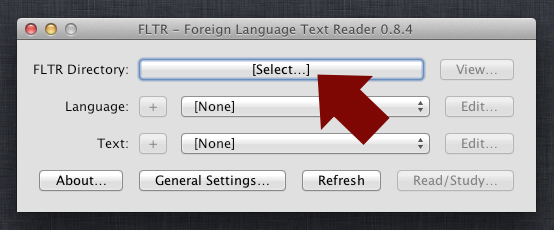
\includegraphics[scale=0.6]{image/images-017.png}

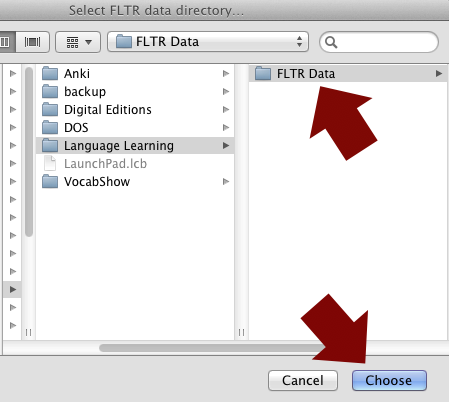
\includegraphics[scale=0.6]{image/images-019.png}

现在创建一个新的语言。(+).在下面的文字中,我们称这种语言为 "XXX"。语言设置将被保存在 "XXX\_Settings.csv "中。

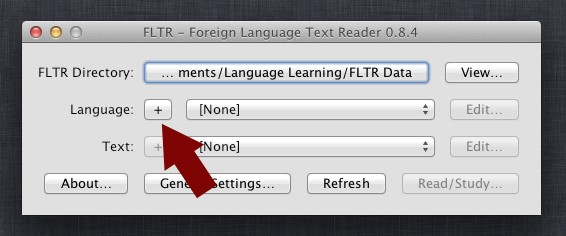
\includegraphics[scale=0.6]{image/images-021.png}

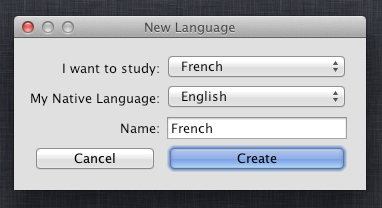
\includegraphics[scale=0.6]{image/images-023.png}

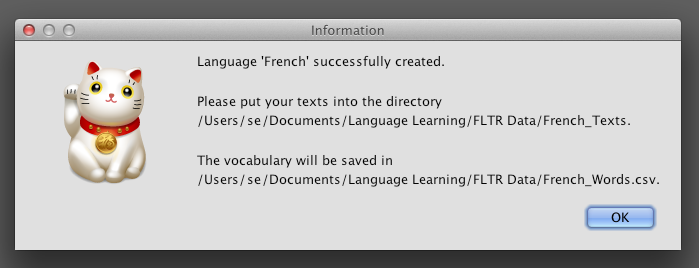
\includegraphics[scale=0.6]{image/images-024.png}

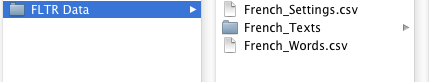
\includegraphics[scale=0.6]{image/images-026.png}

现在做\nameref{FLTR语言设置}。


\chapter{FLTR语言设置}
\label{FLTR语言设置}
语言设置将被保存在 "XXX\_Settings.csv "中,其中XXX是语言。

格式:关键词-值,TAB分隔,不含引号,UTF-8编码。

如果你创建一个新的语言,一个带有默认设置的 "XXX\_Settings.csv"文件将被自动创建。这个默认值对大多数欧洲语言(包括希腊语和西里尔文字)都是可以的。
DictionaryURL1应该被纠正或改变。可以添加第二个和第三个字典。

\lstset{showstringspaces=false} % https://tex.stackexchange.com/a/54185/264374
\begin{lstlisting}
FLTRLANGPREFS
charSubstitutions  ́='|`='|’='|‘='|′='|‵='
wordCharRegExp \-\'a-zA-ZÀ-ÖØ-ö\u00F8-\u01BF\u01C4-\u024F\u0370-\u052F\u1E00-\u1FFF
makeCharacterWord 0
removeSpaces 0
rightToLeft 0
fontName Dialog
fontSize 20
statusFontName Dialog
statusFontSize 15
dictionaryURL1 http://translate.google.com/?ie=UTF-8&sl=xx&tl=yy&text=###
wordEncodingURL1 UTF-8
openAutomaticallyURL1 1
dictionaryURL2 http://glosbe.com/xx/yy/###
wordEncodingURL2 UTF-8
openAutomaticallyURL2 0
dictionaryURL3
wordEncodingURL3 UTF-8
openAutomaticallyURL3 0
exportTemplate $w\t$t\t$s\t$r\t$a\t$k
exportStatuses 1|2|3|4
doExport 1
\end{lstlisting}

该文件必须以包含 "FLTRLANGPREFS "的一行开始。



这些设置可以通过 "Language Settings... "轻松修改。




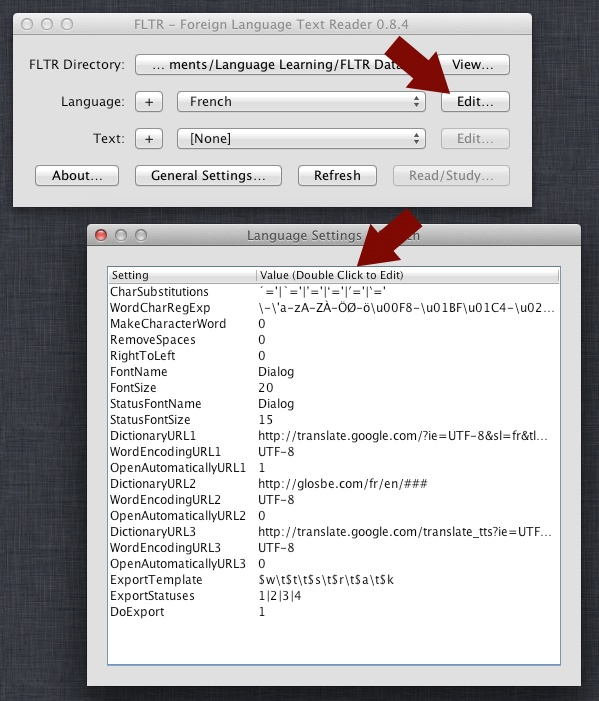
\includegraphics[scale=0.6]{image/images-028.png}

\renewcommand{\arraystretch}{1.3}%https://tex.stackexchange.com/a/159260/264374
\begin{table}[htbp]
\centering
\begin{tabularx}{\textwidth}{|X|X|X|}
\hline
	key & 默认情况下 &解释 \\ \hline
	charSubstitutions & ́='|`='|’='|‘='|′='|‵=' &字符替换的清单。这些主要是为了避免像撇号这样的类似字符在你的词汇中造成问题 \\ \hline
\iffalse
	wordCharRegExp &\makecell{ \textbackslash-\\
	\textbackslash a-z \\ A-Z \\ À-Ö \\ Ø-ö \\\textbackslash u00F8-u01BF \\ \textbackslash u01C4-u024F \\ \textbackslash u0370-u052F \\ \textbackslash u1E00-u1FFF
	}
	& 一个字符列表或字符范围"x-y" ,定义了一个词中的所有字符, 例如 \lstinline{English: "a-zA-Z", German: "a-zA-ZaöüÄÖÜß", Chinese: "一-龥" or"\u4E00-\u9FA5"}。如果你不希望'和-作为单词的一部分。删除 \textbackslash - 和/或 \textbackslash '。另见: : \url{http://tinyurl.com/cbpndlt}(重要的是:在LWT中,Unicode范围被定义。以\lstinline{\x{....}-\x{....}},在FLTR 中你必须指定。\lstinline{\u....-\u....}..........!) \\\hline
\fi
	makeCharacterWord & 0 & 1   针对中文、日文,否 则 0 \\ \hline
	removeSpaces &  0& 1     针对中文、日文,否 则 0 \\ \hline
	rightToLeft & 0 & 1    适用于阿拉伯语、希伯来语、乌尔都语等,否则   0 \\ \hline
	fontName & Dialog & 用于文字显示的字体名称。你必须选择一种能正确显示该语 言字符的字体。 \\ \hline
	fontSize & 20 & 文本显示的字体大小 \\ \hline
	statusFontName & Dialog & 文本状态行的字体名称。 \\ \hline
	statusFontSize & 15 & 文本状态行的字体大小 \\ \hline
	dictionaryURLl & http://translate.google.com/?ie=UTF-8\&sl=xx\&tl=yy\&text=\#\#\# & 词典网址1号或带参数的命令, 调用已安装的词典查询程序  (见  \nameref{与字典查询软件整合})。字的占位符必须给出 \#\#\# 。 \\ \hline
	
	wordEncodingURLl & UTF-8 & URL 1中的单词\#\#\# 的编码 \\ \hline
	openAutomaticallyURLl & 1 & 1=链接1或Cmd 1在点击单词时自动打开 \\ \hline
	dictionaryURL2 & http://glosbe.com/xx/yy/\#\#\#  & 词典URL或命令2 \\ \hline
	
	wordEncodingURL2 & UTF-8 & URL 2中的单词\#\#\# 样的编码 \\ \hline
	openAutomaticallyURL2 & 0 & 1=链接2或Cmd 2在点击单词时自动打开 \\ \hline
	dictionaryURL3 &  & 词典的URL或命合编号3 \\ \hline
	wordEnc。dingURL3 & UTF-8 & URL 3中的单词\#\#\# 的编码 \\ \hline
		
	openAutomaticallyURL3 & 0  & 1=点击单词时自动打开链接3或Cmd 3 \\ \hline

exportTemplate & \$w\textbackslash{}t\$t\textbackslash{}t\$s\textbackslash{}t\$r\textbackslash{}t\$a\textbackslash{}t\$k & 定义词汇导出XXX\_Export.txt或单个词汇导出的编写方式的模板,见VocabularyFile和/或ReviewEditVocabulary。\\ \hline

	exportStatuses & 1|2|3|4 &状态列表,只有具有这些状态的词被导出到XXX\_Export.txt中。\\ \hline
doExport & 1 & 1=总是写一个词汇导出文件XXX\_Export.txt,0=不导出 \\ \hline
\end{tabularx}
\end{table}

注:如下的行因为搞不定,引用原 pdf。

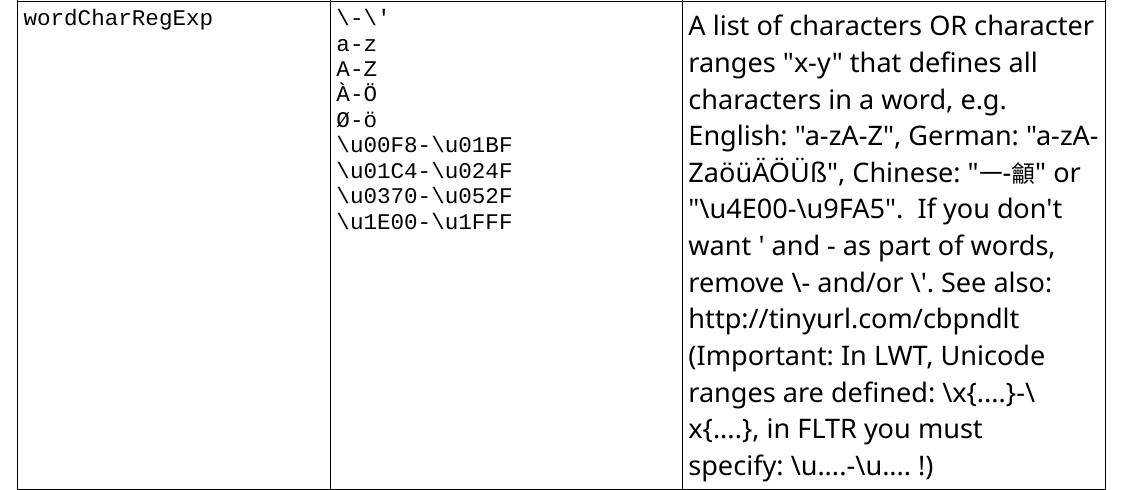
\includegraphics[width=\textwidth]{image/table2.png}


\chapter{与字典查询软件整合}\label{与字典查询软件整合}
\begin{bclogo}[logo=\bcattention, noborder=false, barre=none]{警告!} % https://tex.stackexchange.com/a/53251/264374

本章仅适用于有经验的用户。

你应该 知道如何在终端中用路径和参数调用一个程序。在你开始之前备份你的数据。彻底测试一切。
\end{bclogo}

在上一章中,你学会了如何通过浏览器从网站上打开字典条目。

除了调用网站,还有其他来源可以获得外国单词或表达方式的翻译,如 \goldendict、\translateshell 等词典查询软件。这些应用程序必须单独下载和安装。

那么,如何自动启动这样一个字典查询软件,并显示你要找的某个词的翻译?

我们必须区分两种类型的软件。

\begin{itemize}
    \item  GUI(图形用户界面)软件,在一个窗口中显示其结果。
例如:\goldendict
    \item 将其结果以文本形式写在终端窗口的软件。
例如:\href{https://github.com/soimort/translate-shell}{translate-shell}
\end{itemize}
 
两者都可以用FLTR的点击单词来启动。

在你开始在FLTR中定义一个新的字典查询软件之前,你应该\textbf{备份你的数据}。这样,如果出了问题或不工作,你可以随时回去。

你也\textbf{不应该为一种语言定义一个以上的}字典查询软件。另外两个可以是网站的URL。

你必须知道\textbf{如何调用你的字典查询软件来查询某种语言的词汇}。


\section*{一些例子}(WORD是搜索的词)。

Linux上的 \goldendict。

\lstinline{goldendict "WORD"}

Windows上的 \goldendict。

\lstinline{"C:\textbackslash Program Files (x86)\textbackslash GoldenDict\textbackslash GoldenDict.exe"  "WORD"}

在Linux上 \translateshell (法语→英语,结果简短)。


\lstinline{trans -b fr:en "WORD"}


在Linux上 \translateshell (法语→英语,详细结果)。


\lstinline{trans -no-ansi fr:en "WORD"}


你在字段dictionaryURL1、dictionaryURL2或dictionaryURL3的语言定义中定义启动命令。

如果这些字段的内容以http:// 或 https:// 开始,FLTR将启动你的浏览器并打开给定的网站URL。
如果没有,它将把内容解释为启动一个字典查询软件的命令。

\textbf{该定义必须采用特殊格式。}

\lstinline{程序路径|参数-1|参数-2|...|...|参数-n [&]}



这种格式可能看起来有点奇怪,但它的好处是你不必摆弄引号和/或转义字符。不要使用单引号或双引号或转义空间等!

所搜索的词必须以\#\#的形式给出,不加引号。

如果程序是一个没有文本输出的GUI程序(即输出将显示在GUI程序的一个窗口中),则必须在结尾处给出可选的\&。其结果也是,FLTR不会等到程序结束。它与FLTR并排运行。

如果你没有在最后给出\&,程序应该把翻译写成文本(例如在终端窗口),并且必须在之后结束。这个程序输出显示在FLTR内一个特殊的结果窗口中,通过"鼠标中点",可以很容易地对翻译进行标记(如双击)并复制到FLTR术语窗口的翻译栏中。

如果该程序不结束,它将阻止以下请求。那么你必须点击KILL按钮来解决这种情况。


\textbf{上述例子必须在语言设置 "dictionaryURL1, -2, -3 "中指定如下。}

Linux上的\goldendict GUI程序)。

\lstinline{goldendict | ### &}

Windows上的\goldendict (GUI程序)。

\lstinline{C:\Program Files (x86)\GoldenDict\GoldenDict.exe | ### &}

在Linux上\translateshell(法语→英语,结果简短,文本输出)。

\lstinline{trans | -b | fr:en | ###}

在Linux上\translateshell(法语→英语,详细结果,文本输出)。

\lstinline{trans | -no-ansi | fr:en | ###}

\textbf{最后说明:}

由于无法获得苹果机器,这一功能无法在macOS下测试。

\translateshell 在Windows下不可用,但可能在Windows Subsystem for Linux(WSL)中可以运行。这还没有经过测试。一般来说,Windows下的非GUI程序如果必须在Windows终端内运行,会有很多编码和其他问题。

\textbf{再一次:}


在尝试将字典查询软件整合到FLTR之前,请对你的数据进行备份。


\textbf{示例截图(Linux):}

定义的截图 - \goldendict 。

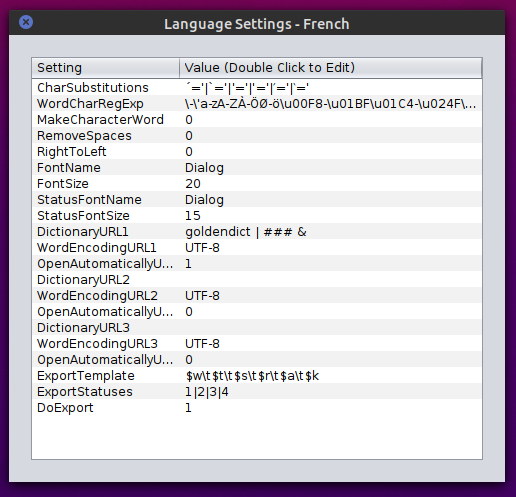
\includegraphics[scale=0.5]{image/images-030.png}

使用截图 - \goldendict 。

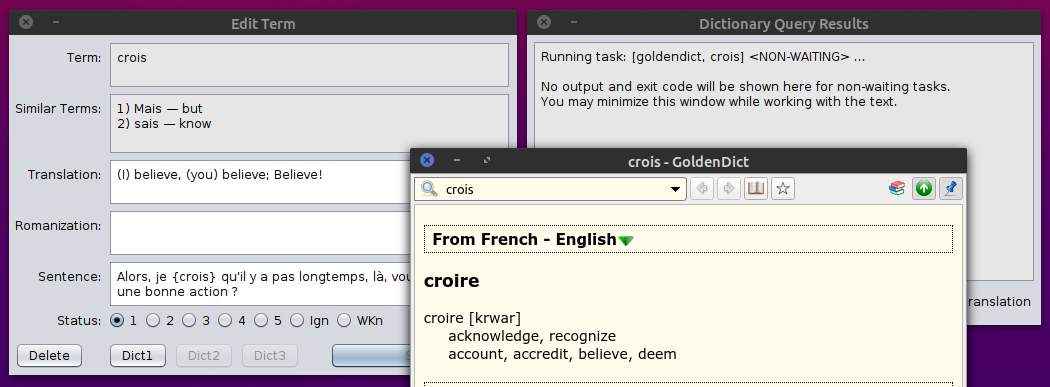
\includegraphics[scale=0.4]{image/images-031.png}


使用情况的截图-- \translateshell。

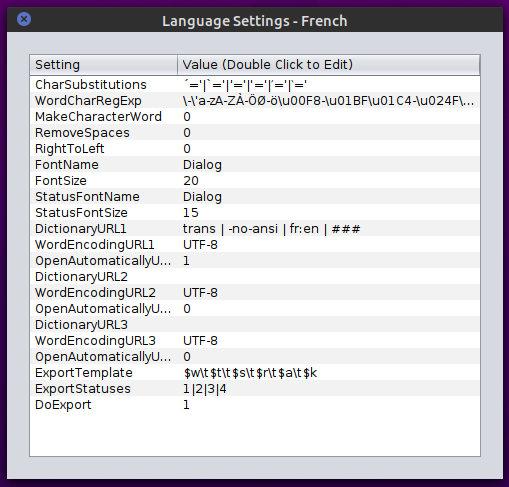
\includegraphics[scale=0.6]{image/images-032.png}


使用情况的截图-- \translateshell。

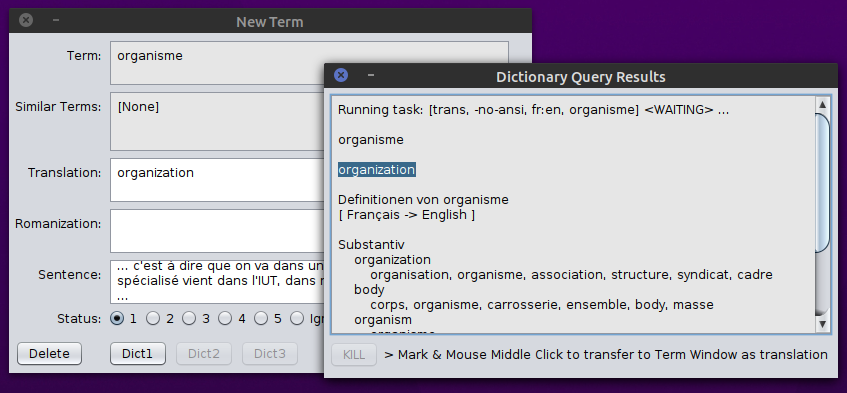
\includegraphics[scale=0.4]{image/images-033.png}


\chapter{常规设置}
\label{常规设置}
FLTR的一般设置(文本区域大小、窗口位置、外观和感觉、字体大小系数、弹出菜单类型、颜色)被保存在当前用户主目录下的".fltrprefs "文件中(该文件在Mac/Linux/Unix上是隐藏的)。

格式:关键词-值,以TAB为界,不带引号,UTF-8编码。该文件必须以 "FLTRPREFS"一行开始。

目前,用户可以改变的唯一有趣的数据(只需点击 "General Settings...")是,见屏幕截图。

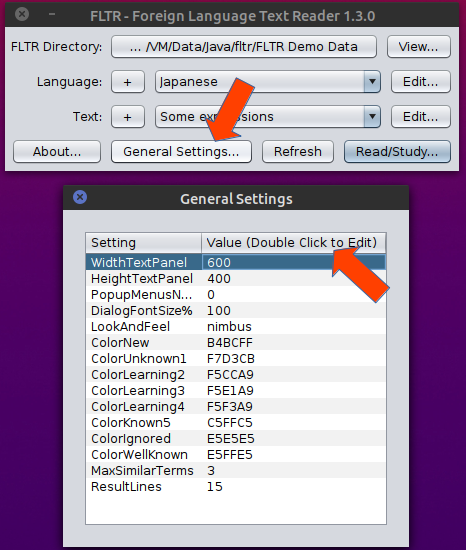
\includegraphics[scale=0.8]{image/images-034.png}

\begin{itemize}
    \item 文本窗口中的文本面板的宽度和高度。默认值是600 x 400。由于上网本的屏幕尺寸较小,所以它被设置得相当小。如果你想要一个更大的文本区域,只要把这些数字弄大,例如1000 x 700。但请注意,你还需要为浏览器窗口、数据输入窗口和媒体播放器程序窗口提供屏幕空间。

     \item 文本区弹出式菜单可以嵌套(旧版本=1)或不嵌套(新版本,=0,默认)。
     \item 对话框字体大小(百分比),默认=100,允许的值范围。75 ... 150 \%.在某些平台和某些外观上,这个值可能被忽略。自己去找吧。特别是在Windows上。在外观和感觉=系统的情况下,110或120\%是一个好的值。更改后必须重新启动程序。
     \item 外观和感觉。可能的值是:系统(默认)、Nimbus(字体大小必须是100\%)或金属。使用你喜欢的任何东西。更改后必须重新启动程序。
     \item  不同术语状态的背景颜色的HTML(十六进制或十六进制)颜色代码(前面没有 "\#")。你可以通过 \href{https://htmlcolorcodes.com/} 找出代码。如果你删除了一个颜色代码,将自动设置为默认值。
     默认情况下。
     \begin{lstlisting}
New B4BCFF
Unknown1 F7D3CB
Learning2 F5CCA9
Learning3 F5E1A9
Learning4 F5F3A9
Known5 C5FFC5
Ignored E5E5E5
WellKnown E5FFE5
     \end{lstlisting}

     \item 术语窗口 "MaxSimilarTerms"中显示的类似术语的数量可以从0到10设置。这个功能可以通过设置为零来关闭。类似术语的最大数量是10,默认值是3。
     \item 结果窗口中的行数(=调用外部字典查询软件的结果)对应的变量 "ResultLines" 在 5-50 之间设置,默认为15。
\end{itemize}

\chapter{阅读文本,创造和编辑词语或表达方式}\label{阅读文本,创造和编辑词语或表达方式}
你有两种可能性来保存你正在学习的语言的文本。

\textbf{方法一:}

将一些文本(例如来自互联网)复制到剪贴板(通过Ctrl+C或Cmd+C)。

现在点击 "文本:"右边的(+)。文本将自动从剪贴板上粘贴。你必须提供一个文本名称并点击(保存文本)。

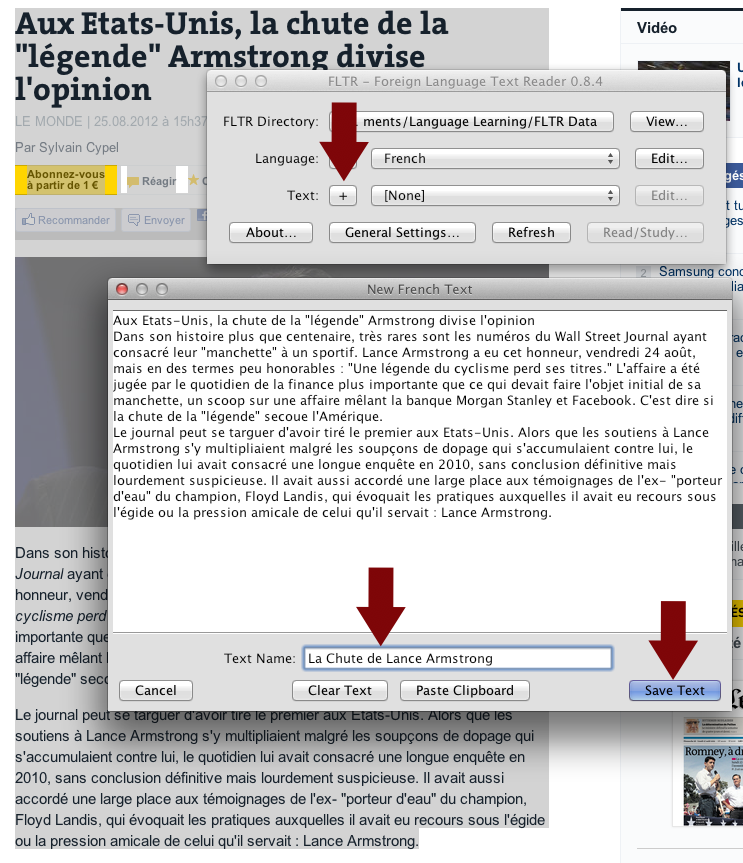
\includegraphics[scale=0.5]{image/images-035.png}

\textbf{方法二:}

保存或复制一些你想研究的文本到FLTR数据目录下的新目录 "XXX\_Texts"。请使用".txt "文件扩展名,并在文本编辑器中保存为UTF-8编码,如Notepad++(Win)或TextWrangler(Mac)。如果您使用OpenOffice、LibreOffice等文本处理器,请保存为"编码文本 "并选择UTF-8编码和CRLF换行。

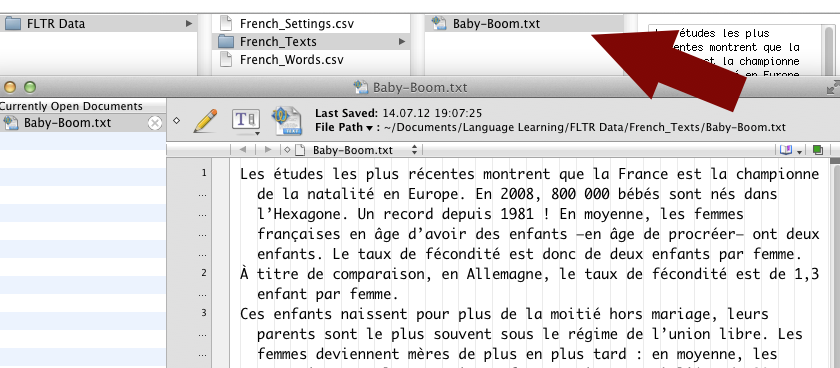
\includegraphics[scale=0.5]{image/images-037.png}

点击(刷新),使程序知道新保存的文本,然后选择一种语言,并选择一个文本,点击(开始学习...)。

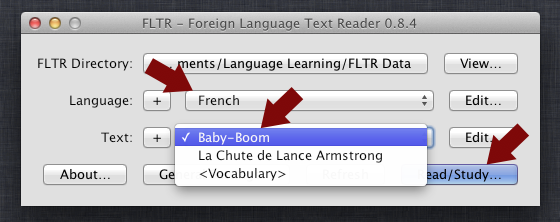
\includegraphics[scale=0.6]{image/images-039.png}

每个词或多词表达(都称为 "术语")都有一个状态,用一种颜色指定。

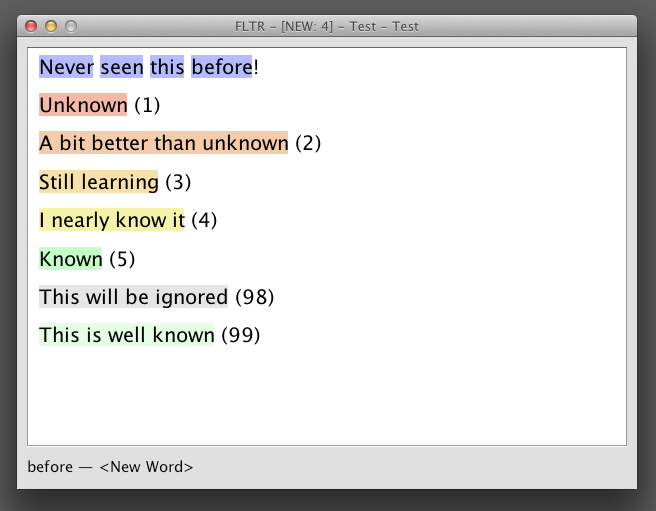
\includegraphics[scale=0.6]{image/images-041.png}

\textbf{将鼠标悬停在一个术语上:}你可以看到该术语的翻译、罗马化(如果有的话)和状态。

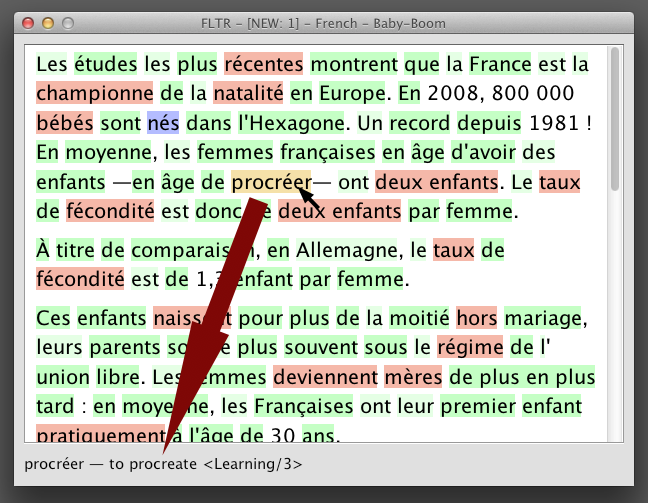
\includegraphics[scale=0.6]{image/images-042.png}

左键点击一个蓝色的(新)术语。网络词典(openAutomaticallyURL...=1)将打开,你可以创建一个新的术语或词汇项。

左键点击一个非蓝色的(存在的)术语。网络词典(openAutomaticallyURL...=1)将打开,你可以编辑该术语。

右键点击一个词:弹出一个菜单,你可以创建或编辑术语,查询字典,改变术语状态,处理基础(隐藏)术语,在浏览器中打开文本,显示每个文本和当前语言的词汇量,保存或导出当前语言的所有术语。

在第一个词上左键单击并按住,移动到最后一个词并松开。一个新的多词表达式将被创建,如果它已经存在,可以对它进行编辑。

如果一个段落的结尾在这样的多字表达式中,它可以被创建和保存,但不会在文本中显示。但它会出现在有这样一个多词表达的文本中,但其中没有段落结尾

限制。术语或多词表达的长度是有限的:最多200个字符。这同样适用于翻译和罗马化
。例句的长度可以达到400个字符。


\chapter{词汇文件}\label{词汇文件}
词汇表将被保存在 "XXX\_Words.csv "中,其中XXX为语言。以前的版本可在
"XXX\_Words.bak "中找到。

格式。以TAB为界,无引号,UTF-8编码。它与LWT TSV导出的格式相同,所以你可以下载你的LWT术语(TSV导出)并替换文件 "XXX\_Words.csv"。

只有字段1至5将被读取。字段2至5是可选的,见默认值。

如果在阅读词汇文件时,同一个词出现了不止一次,那么最后出现的那个词获胜。

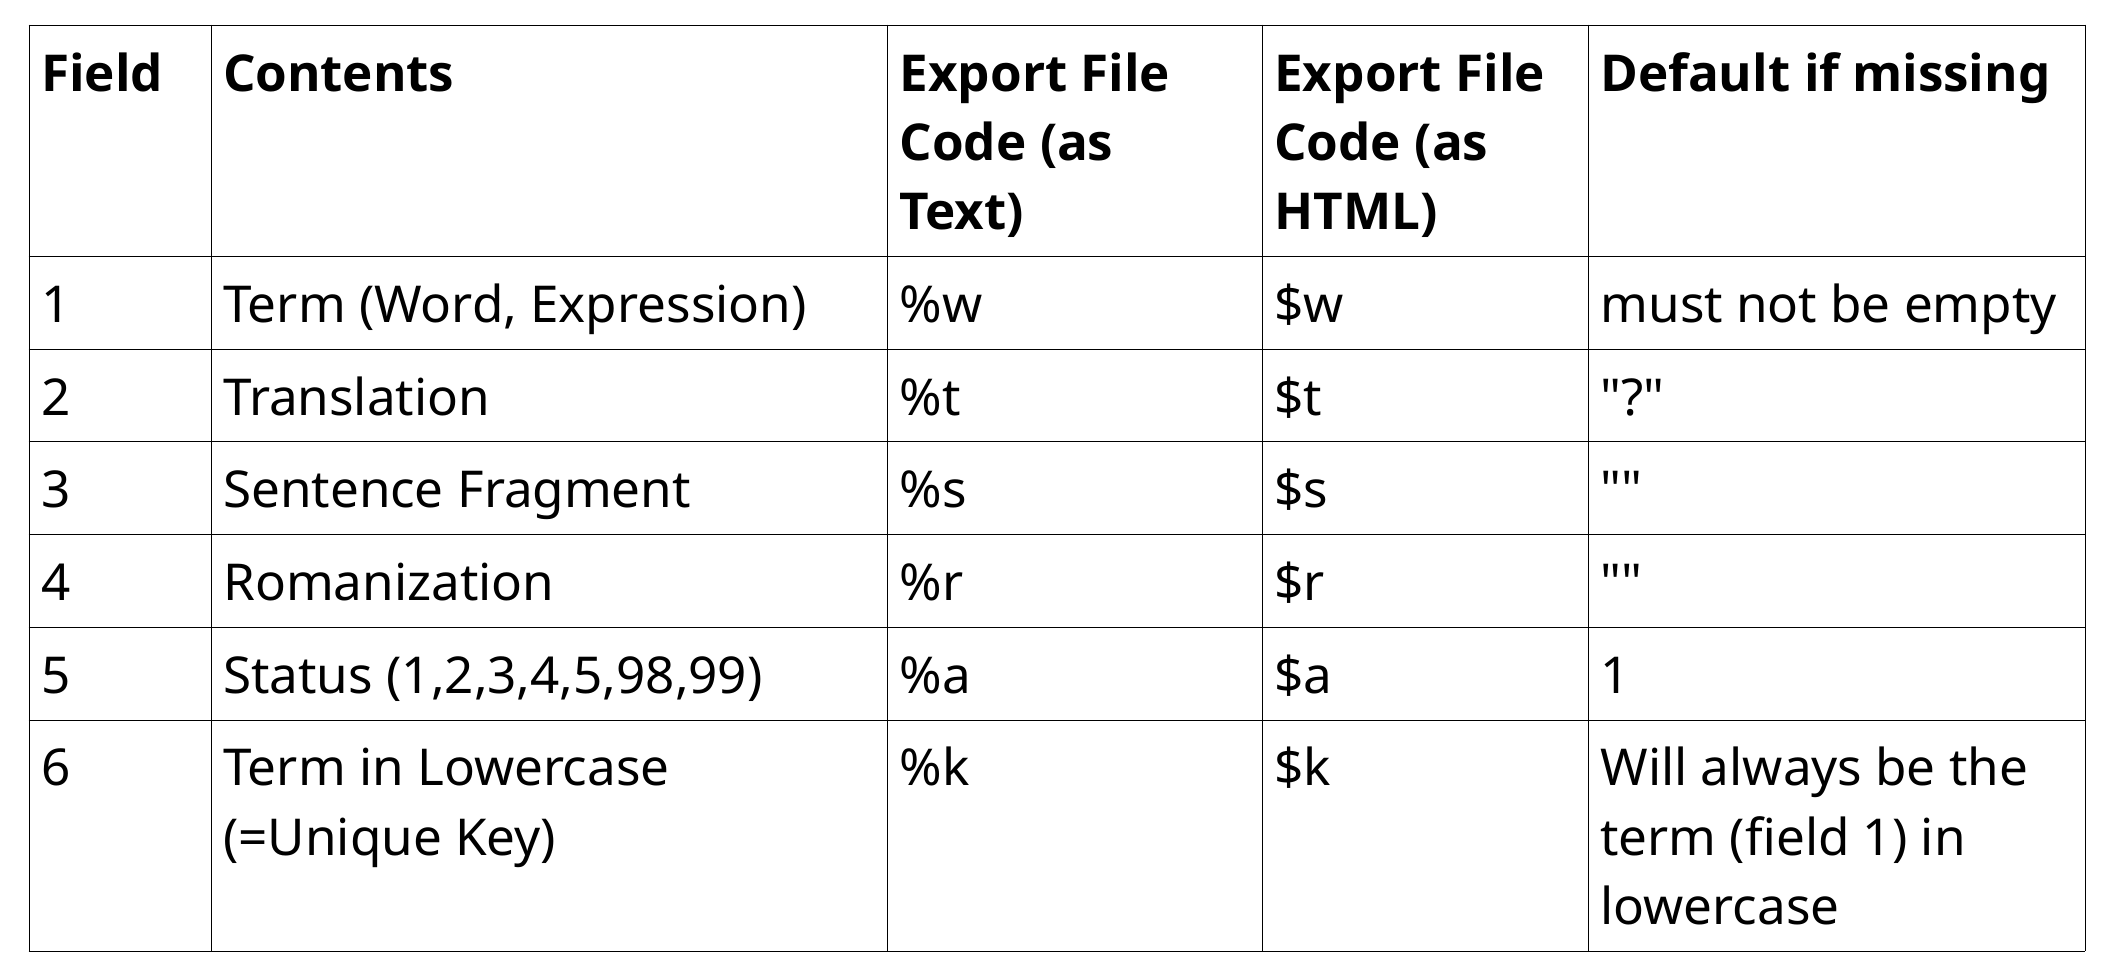
\includegraphics[scale=0.3]{image/table3.png}

在你结束对文本的处理后,如果你对你的词汇做了一些修改,你会被问到是否要保存你的修改。如果你点击(是),完整的词汇表(以及导出文件,如果 "doExport"设置为1)将被保存到磁盘(字段1至6)。

\chapter{输出文件}\label{输出文件}
上述代码(见表)是 "导出词汇 "模板 "exportTemplate "的占位符。

如果在语言设置中 "doExport "被设置为1,则会创建导出文件。它包含所有在语言设置"exportStatuses "中的状态列表中具有当前状态的词汇项。

导出文件XXX\_Export.txt可以很容易地(重新)导入Anki(使用\$.占位符!)。

\%w, \%t, \%s, \%r, \%a, \%k是原始数据的占位符,见表。

\$w, \$t, \$s, \$r, \$a, \$k是带有转义的HTML特殊字符的数据占位符(< = \&lt;, > = \&gt;, \& =
\&amp; " = \&quot;, 见表。

要输入一个TAB字符,请使用\textbackslash t。

要输入一个换行字符,请使用\textbackslash n。

要输入美元、百分号或反斜杠:使用\$\$、\%\%或\textbackslash\textbackslash。有一些特殊的占位符用于cloze测试。

\%c = 句子,其中的{...}被"{***}"所取代。

\$c = 像\%c一样,但转义了HTML特殊字符。

\%d = 句子中的{...}被"{***翻译***}"所取代。

\$d = 类似于\%d,但转义为HTML特殊字符。

\textbf{输出文件实例1}

\begin{lstlisting}
exportTemplate = $w\t$t\t$s\t$r\t$a\t$k
EXPORT (escaped HTML special characters):
Word[TAB]Translation[TAB]Sentence[TAB]Romanization[TAB]StatusCode[TAB]Key
\end{lstlisting}

\textbf{输出文件示例2}

\begin{lstlisting}
exportTemplate = $w\n$t\n$s\n$d\n$a\n$k\n---
EXPORT (escaped HTML special characters):
Word<br>
Translation<br>
Sentence With {Word}<br>
Sentence With {***Translation***}<br>
StatusCode<br>
Key<br>
---
\end{lstlisting}


\chapter{复习和编辑词汇}\label{复习和编辑词汇}
当选择一个文本时,你会看到一个条目<词汇表>。

如果你选择了这个特殊的条目,并点击(开始学习......),你会看到 "词汇过滤和排序选项"。

你现在可以对你的词汇进行过滤、排序和限制,而且这些词汇的选择现在可以...

\begin{itemize}
    \item 像文本一样复习/编辑。
     \item 在浏览器中复习/测试。
     \item 或根据导出模板保存为文本文件,见 "词汇文件"。
    
\end{itemize}

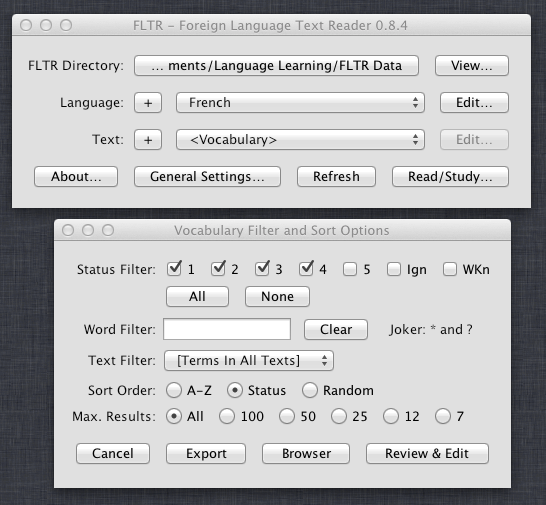
\includegraphics[scale=0.6]{image/images-044.png}

Actions:

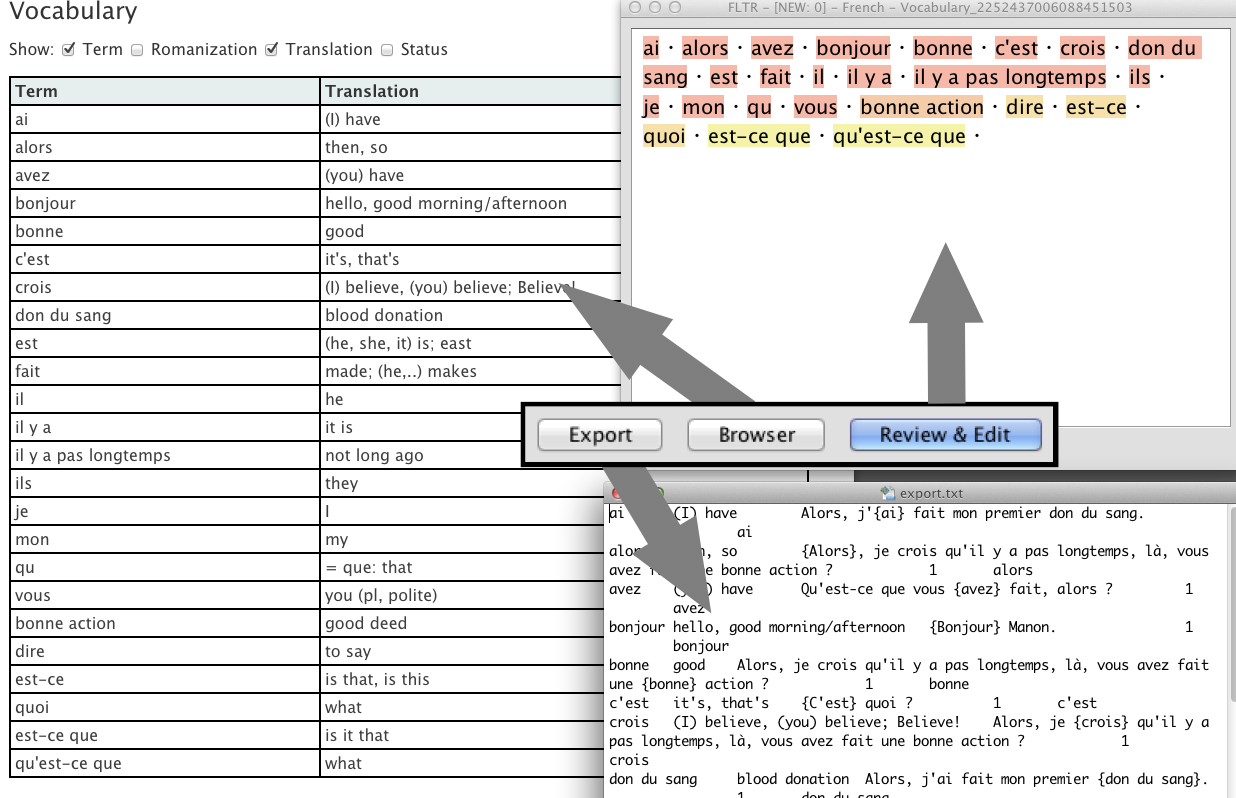
\includegraphics[scale=0.3]{image/images-045.png}


\chapter{常见问题解答(FAQ)}\label{常见问题解答(FAQ)}
Q:
有些字符不显示,或显示错误。

A:
改变语言设置中的字体。试试"Dialog",或将其设置为适合你所学语言的字体,或安装Unicode字体并在语言设置中设置。\\
另见 \url{http://en.wikipedia.org/wiki/Unicode_font}

Q:
音频播放器在哪里?

A:
没有。只要使用你最喜欢的音频播放器:iTunes、Winamp、VLC等。 如果你是一
个中高级的语言学习者,你会经常使用FLTR而不听音频,只是因为不存在相关的音频
文件。

\chapter{比较类似软件(FLTR, LWT, LingQ)}
\label{比较类似软件(FLTR, LWT, LingQ)}
\renewcommand{\arraystretch}{1.3}%https://tex.stackexchange.com/a/159260/264374
\begin{table}[htbp]
\centering
\begin{tabularx}{\textwidth}{|X|X|X|X|}
\hline
特点 &FLTR & LWT& LingQ\\\hline
编程语言 &Java &PHP, JavaScript &未知,可能是PHP、JavaScript\\ \hline
应用类型& 桌面应用程序 &网络应用程序 &网络和移动应用程序\\\hline
数据存储& 文本和TSV文件& MySQL数据库& 未知,可能是MySQL数据库\\ \hline
开放源码& 是 &是 &否\\ \hline
许可证&MIT &公共领域 &专有的\\ \hline
环境需求& Java运行时& 本地或远程网络浏览器,服务器&网络浏览器\\ \hline
安装& 解压ZIP并运行 &网络服务器安装& 无\\ \hline
速度& 非常快& 在本地相当快& 中等到缓慢,取决于互联网连接和服务器负载\\ \hline
语言& 所有Unicode(包括从右到左的)。& 所有Unicode(包括从右到左的)。& 目前(2021年)有 24种语言\\ \hline
音频支持& 不(使用你的个人电脑的播放器)&是的,HTML5播放器& 是的,HTML5播放器\\ \hline
文本标签支持& 没有& 是& 是\\ \hline
文字归档& 没有,但只要将文本移入/移出FLTR文本目录即可。& 是& 是\\ \hline
术语标签支持 &没有 &是 &是\\ \hline
文本管理& UTF-8格式的文本文件& 上传至数据库& 上传,必须是付费会员\\ \hline
导入内容& LWT:简单(通过 "导出所有术语(TSV)")。其他:例如,通过电子表格&灵活的导入功能&
 简单导入功能,必须 是付费会员\\ \hline
导出内容& 灵活,通过模板&Anki和TSV& 简单的CSV,必须是付费会员\\ \hline
最多词条数 & 无限制& 无限制& 免费会员:20,付费会员;无限制\\ \hline
最多词组词数& 不限,但最多200个字符 &  9 & 不详\\ \hline
显示相似术语 &  是的,最多10个。& 是& 没有\\ \hline
查看/编辑词条 &  是的,通过右键点击 & 是的,在显示模式切换后 &  是的,在点击\\ \hline
测试 &  无 , 使 用 Anki 或其他 闪 卡程序&  是 &  是\\ \hline
统计数据 & 只统计字 & 是 &  是\\ \hline
费用 & 免费 &  免费 & ≈10美元/月\\\hline
\end{tabularx}
\end{table}

\chapter{版本历史}
\label{版本历史}
0.8.9(2019-03-20)\\
转换成了Java 1.8。
现在支持具有安全(https://...)和不安全(http://...)网络协议的外部词典。
"FLTR for macOS + Apple's Java 1.6 "已不再适用,因为现在是在Java 1.8中进行开发
。请看安装。
一些小的变化。

0.8.10(2020-07-17)\\
在默认浏览器中打开一个URL的逻辑已经被修改。

1.0.0(2020-10-03)\\
转移到另一个Sorceforge项目。
一些小的修正(网络链接,打开外部程序的逻辑,关于信息)。

1.1.0(2021-05-25)\\
现在可以编辑背景颜色来显示不同的级别。现在可以用鼠标在术语窗口中进行粘贴、
复制、剪切操作。删除了在术语窗口中显示类似术语的功能(在以前的版本中没有价
值和功能)。
现在可以通过右键弹出菜单保存和导出工作中的所有术语。
期限窗口的一些改进。

1.2.0(2021-05-30)\\
在术语窗口中可以再次显示类似的术语,现在可以进行配置。现在显示在一个不可
编辑的文本字段中,最多可显示3行。这个功能可以通过将 "MaxSimilarTerms "偏好设
置为零来关闭。类似术语的最大数量是10,默认值是3。 你可以从这个文本框中复制
和粘贴文本。
术语窗口中的术语现在无法编辑。

1.3.0(2021-06-09)\\
现在可以将FLTR与GoldenDict、translate-shell等字典查询软件整合。见 "与字典查
询软件的整合 "一章。对 "我知道所有 "的操作实施确认对话框。

1.4.0(2021-06-14)\\
现在,文本中的最后阅读位置会被自动保存,并在你阅读时恢复。再次打开它。但是,在改变文本字体、文本字体大小或文本面板宽度/高度后,这种改变后的阅读位置可能是错误的。

\end{document}
